\chapter{Introduction}

As electronic devices keep shrinking in size, metallic nanostructures such as nanofilms and nanowires have gained increasing importance in a wide range of electronic applications, such as high-density interconnects, sensors \cite{walter2002}, and flexible electronics \cite{facchetti2010}. The reduction in size of device components increases computational power, but at the same time increases energy density and localised heating. 
Therefore, in order not to compromise the device's performance, it is essential to dissipate this heat as effectively as possible. Consequently, understanding and controlling the thermal conductivity of metallic nanostructures has become a topic of significant scientific interest. 

That being said, it should come as no surprise to find in the literature that in the last decades, there has been extensive discussion regarding thermal transport in metallic nanostructures \cite{lin2013, feng2009thin, CahillNanoscale2003}. Both experimental and theoretical findings indicate the presence of a size effect: the thermal conductivities of metallic nanostructures are lower than those of their bulk counterparts and vary with the dimensions of the nanostructures. This size effect is believed to be the result of several factors, including surface and grain boundary scattering, altered electron-phonon interactions \cite{Zhang2006}, and reduced local coordination sites.

\begin{figure}[H]
    \centering
    \includegraphics[width=1\linewidth]{photos/nanowires.jpg}
    \caption{Scanning Electron Micrographs (SEMs) of palladium nanowires (A and B) prepared by electrodeposition from aqueous 2.0 mM Pd(NO$_3$)$_2$, 0.1 M HClO$_4$, E$_{dep}=+0.3$ V/SCE, t$_{dep}=900$ s \cite{walter2002}.}
    \label{fig:nanowires}
\end{figure}

Gold (Au), in particular, serves as an ideal reference material for studying thermal transport in metals due to its high thermal conductivity, chemical stability, and widespread use in electronic components such as interconnects and contacts. The thermal conductivity of bulk gold at room temperature is about 317 W/mK, making it one of the best conductors. However, when reduced to nanoscale dimensions, gold exhibits a significant reduction in thermal conductivity \cite{Anderson2021}, with the exact contribution of phonons remaining a matter of debate \cite{Sawtelle2019}. Some studies suggest that the phonon contribution is negligible compared to the electronic one, whereas others indicate that phonons can contribute substantially to heat transport, especially in nanostructured or porous systems \cite{Mason2020}.\bigskip

Then, understanding the phonon contribution is critical, particularly in light of technological applications where nanoscale structuring could change heat transport. To gain insight into thermal transport mediated by phonons in gold nanostructures, computational methods such as molecular dynamics simulations combined with the Green-Kubo formalism provide a powerful framework, allowing for a detailed analysis of how size, porosity, and structure influence thermal conductivity.

\section{State-of-the-art}
In this section, we provide a brief overview of thermal transport in gold, highlighting the contributions of both electrons and phonons to heat conduction. We also introduce some representative nanoscale systems, which will serve as the focus for the subsequent analysis. This context aims to establish the fundamental concepts necessary to understand how thermal conductivity is calculated and how dimensions and structural effects influence heat transport in bulk and nanostructured gold, as well as to provide context for the work presented in this thesis.

\subsection{Gold Conductivity}
In bulk gold, thermal conductivity is dominated by electronic contributions, while the phononic component is generally small due to strong electron–phonon scattering and the relatively short phonon mean free paths. At room temperature, electrons account for the vast majority of heat transport, in agreement with the Wiedemann–Franz law \cite{Wiedemann_Franz_law}, which links electrical and thermal conductivity in metals through electronic diffusion. The lattice contribution is often considered negligible in comparison to the electronic one. In fact, several studies suggest that the phononic contribution to the thermal conductivity of bulk gold corresponds to approximately 1-2\% of the total conductivity of gold, which has a well-established value of 317 W/mK, corresponding to a value of roughly 3-6 W/mK. \bigskip

However, recent theoretical and experimental investigations have shown that the phononic contribution, although modest in bulk, is not negligible. First-principles calculations indicate that phonons with mean free paths in the range of a few nanometres can still provide a finite lattice thermal conductivity, and that the balance between phononic and electronic transport is sensitive to scattering rates and microstructural features. Moreover, deviations from Wiedemann–Franz behaviour have been reported in nanoscale gold structures \cite{Hu2021}, suggesting that the simplistic picture of purely electronic transport becomes insufficient when spatial confinement or structural disorder are present.\bigskip

When gold is reduced to the nanoscale, in the form of thin films, nanowires or porous architectures, the situation changes considerably. Size effects such as increased surface-to-volume ratio, boundary scattering, enhanced disorder, and the emergence of complex interfaces all reshape the microscopic pathways responsible for energy transfer and lead to a substantial reduction of the electronic thermal conductivity. In such systems, the reduced electronic contribution amplifies the relative importance of the ionic one, which can become comparable to or even exceed the electronic part depending on the geometry details. This has led to an active debate in the literature, with some studies reporting an almost negligible phonon contribution and others demonstrating that phonons can play a significant role in nanostructured or disordered gold \cite{Hu2021}.


\subsection{Computing electronic conductivity}
The electronic thermal conductivity in gold can be evaluated by combining transport theory with measurable electrical properties. In metals, heat is primarily carried by conduction electrons, whose transport is well described within the framework of the free-electron or quasi-free-electron model. Under this approximation, the electronic thermal conductivity $k_e$ is commonly obtained through the Wiedemann–Franz law:
\begin{equation}
    k_e=L \sigma T ,
\end{equation}

where L is the Lorenz number,  $\sigma$ the electrical conductivity, and T the absolute temperature. For bulk gold at room temperature, the Lorenz number is close to the Sommerfeld value $L_0=2.44\times 10^{-8}W\Omega / K^2$, reflecting the dominance of elastic electron scattering. Thus, accurate measurement or estimation of $\sigma$ directly yields. The temperature dependence of $k_e$ follows from the interplay between electron–phonon scattering and impurity scattering: as temperature increases, enhanced phonon scattering reduces the electronic mean free path, leading to a decrease in both $\sigma$ and $k_e$.\bigskip

In nanostructured or porous gold, the situation becomes more complex. Size confinement, grain boundaries, and surface roughness introduce additional scattering channels, often breaking the simple Wiedemann–Franz proportionality. The Lorenz number may deviate significantly from $L_0$. As a consequence, estimating the electronic contribution to thermal conductivity requires models that incorporate all of these size effects, such as Mayadas–Shatzkes formalisms \cite{mayadas1970}, or experimental techniques such as time-domain thermoreflectance (TDTR) \cite{Jiang2018}.

Another powerful method to model electron transport in such systems is the resistor network approach. In this framework, the system is represented as a network of resistors, where each segment corresponds to a conductive path between neighbouring atoms or grains, with resistance $R = L/(\sigma A)$ determined by the segment length $L$ and cross-sectional area $A$. Porosity, defects, or bottlenecks are naturally included as increased resistances or missing connections. By solving the network using Kirchhoff’s laws, one can estimate the effective electronic conductivity of the entire structure, including the influence of geometry and connectivity. 

Regardless of the research approach, the results confirm that in nanostructured or porous gold, the effective electrical conductivity is strongly reduced. And the closer we get to the nanoscale, the more the electronic conductivity approaches that of phononic conductivity, which becomes increasingly important.


\subsection{Computing phonon conductivity}
While the phononic contribution to thermal conductivity should be small and negligible for bulk materials, this is not the case at the nanoscale. Therefore, understanding and quantifying the lattice contribution to heat transport becomes essential, and dedicated methods are required to capture phonon dynamics, scattering mechanisms, and their dependence on structure and size.

The phononic conductivity can be calculated employing different approaches, which vary in computational cost and physical realism, and best represent different types of materials (perfect crystalline, disordered, nanostructures, etc.). \bigskip

To evaluate the lattice thermal conductivity, an important category of methods is the first-principles approach based on solving the phonon Boltzmann Transport Equation (BTE) \cite{Peierls_1929}. The heat current is expressed in terms of the phonon distribution function $f_{\lambda}$, which at thermal equilibrium follows the Bose–Einstein statistics $f_{0}$. When a temperature gradient is applied, $f_{\lambda}$ deviates from $f_{0}$, and the BTE describes the balance between the diffusive term driven by $\nabla T$ and the phonon–phonon scattering processes. In the steady-state regime ($df_{\lambda}/dt = 0$), this gives rise to the expression:
\begin{equation}
 - v_\lambda\cdot \nabla T + \frac{\partial f_{\lambda}}{\partial T} \Big|_{\text{diffusion}} + \frac{\partial f_{\lambda}}{\partial T} \Big|_{\text{scattering}} =0.
\end{equation}
Within this class of methods, harmonic and (when needed) anharmonic interatomic force constants are computed with ab initio calculations, and the phonon BTE is subsequently solved to obtain the lattice thermal conductivity \cite{Fugallo_2013, Qin_2015}.


A more simplified and computationally light alternative is the Debye–Callaway model \cite{Callaway1959}, in which the lattice thermal conductivity is the sum of three acoustic modes: one longitudinal $\kappa_{LA}$ and two transverse $\kappa_{TA}$ and $\kappa_{TA'}$:
\begin{equation}
    \kappa = \kappa_{LA} + \kappa_{TA} + \kappa_{TA'}.
\end{equation}
However, this method has clear limitations: the Debye-like simplification of the phonon dispersion overestimates the group velocity of high-frequency modes, leading to an overestimation of $\kappa$, especially when optical modes contribute significantly. In fact, the deviation between theoretical predictions and experimental results often originates from the contribution of optical phonon modes, which the Debye–Callaway model does not account for \cite{Zhang2016}.

This class of theoretical approaches is highly effective for ideal periodic crystals, where phonons behave as well-defined wave-like particles; however, when moving to nanoscale objects or systems with significant disorder, defects, finite-size effects, surface scattering, or broken periodicity, these assumptions progressively break down, and the phonon picture itself loses validity.
\bigskip

Another family of methods consists of molecular dynamics (MD) simulations in a non-equilibrium regime, where a temperature gradient is imposed, and the thermal conductivity is measured from the macroscopic response of the system. In addition, combining MD with spectral analysis techniques, information can be obtained not only on total $\kappa$, but also on modal contributions, phonon mean free paths, and conductivity spectrum \cite{Fan_2019}. These approaches are particularly valuable at the nanoscale or in systems with significant disorder, defects, where phonons are not well-defined quasiparticles and wave-like descriptions lose validity. \bigskip

The Green–Kubo (GK) formalism provides a powerful approach to calculate the lattice thermal conductivity $\kappa$ from equilibrium molecular dynamics simulations. The GK method relies on the fluctuation-dissipation theorem, which relates macroscopic transport coefficients to the time correlation of microscopic fluxes. In the case of thermal transport, the lattice thermal conductivity is obtained by integrating the heat flux autocorrelation function (HFACF) over time:
\begin{equation}
    \kappa_{\alpha\beta}=\frac{1}{k_BT^2V}\int_0^\infty \langle J_\alpha(0)J_\beta(t) \rangle dt,
\end{equation}
where $J_\beta(t)$ is the $\beta$-component of the total heat current, $V$ the system volume, $T$ the temperature, and $k_B$ the Boltzmann constant.

This method can safely be extended to nanoscale or disordered systems, where the assumptions of well-defined phonon wave vectors and periodicity break down, as it does not require the definition of phonon modes or the solution of the BTE. Therefore, it can be effectively used alongside Non-Equilibrium Molecular Dynamics (NEMD) methods to provide complementary insights into thermal transport.


\subsection{Nanomaterials}
Nanomaterials are systems whose structural features lie between the atomic and macroscopic scales, from one to a few hundred nanometres. They exhibit physical and chemical properties that deviate strongly from bulk behaviour due to quantum confinement, high surface-to-volume ratios, and enhanced interfacial effects. At these scales, electronic states become quantised, phonon transport is strongly influenced by boundaries and interfaces, and surface atoms with reduced coordination dominate the material’s response.

Thanks to these unique characteristics, nanomaterials play a central role in a wide range of technologies: high-surface-area supercapacitors \cite{Yoon2001CarbonAerogels}, high-power-density batteries \cite{Rolison2009Multifunctional3D}, hydrogen storage \cite{Borup2007Thermoelectrics, DiVece2004}, electromagnetic interference (EMI) shields \cite{Zhao2021}, heat sinks \cite{Busch1984Copper}, ultra-high-field electromagnets \cite{Ashby2000MetalFoams}, and neuromorphic circuits \cite{Profumo2021Neuromorphic}. These applications exploit their high conductivity and porosity, their three-dimensional structure for electronic and mechanical transport, their large internal surface for adsorption, their unconventional electromagnetic response, and the optimisation of thermal conduction, thermal management, and resistive switching capabilities. Among these technologies, resistive random-access memories (ReRAMs) are particularly promising: they store information through resistive switching and can be realised in various architectures, such as metallic nanoparticle assemblies and nanowire networks \cite{TiberiBaletto2024}, ultimately enabling the development of systems capable of mimicking complex brain-like connectivity \cite{Wang2019}. 

Understanding thermal transport in such nanostructures becomes essential. Heat dissipation directly affects device reliability. Accurate control of electron and phonon transport is therefore fundamental for optimising energy-storage materials, catalytic activity, and nanoscale electronic components based on metallic networks. \bigskip


Among nanomaterials, nanopillars are portions of nanowires, nanorods, or nanofilaments positioned between electrodes, as shown in Figure \ref{fig:fil_grow}. They are nanometric columns that combine high surface area with well-defined vertical orientation. These structures offer a wide range of interesting chemical and physical properties, such as better electronic properties \cite{Chou-Yi2023}, increased mechanical durability \cite{Li2024}, and adjustable optical or catalytic characteristics \cite{Fang2025}.

\begin{figure}[H]
    \centering
    \includegraphics[width=0.9\linewidth]{photos/fil_grow.jpg}
    \caption{Bias-assisted electrochemical growth of a gold filament directly at the apex of a conductive AFM tip \cite{Bakhti2016}. The resulting structure is a polycrystalline, mechanically stable and conductive gold nanofilament, with controllable length (from a few tens up to several hundreds of nanometres) and a curvature radius of about 3 nm.}
    \label{fig:fil_grow}
\end{figure}

Metallic nanofoams are a type of three-dimensional porous materials that feature a network of interlinked metallic nanoparticles, creating a highly branched and porous arrangement as shown in Figure \ref{fig:how2nanofoam}. They merge the conventional characteristics of bulk metals, such as excellent electrical and thermal conductivity, with the features commonly seen in nanoarchitectures, including increased surface area, low density, improved catalytic properties, and a high strength-to-weight ratio, making these systems particularly attractive for advanced research. 

\begin{figure} [H]
    \centering
    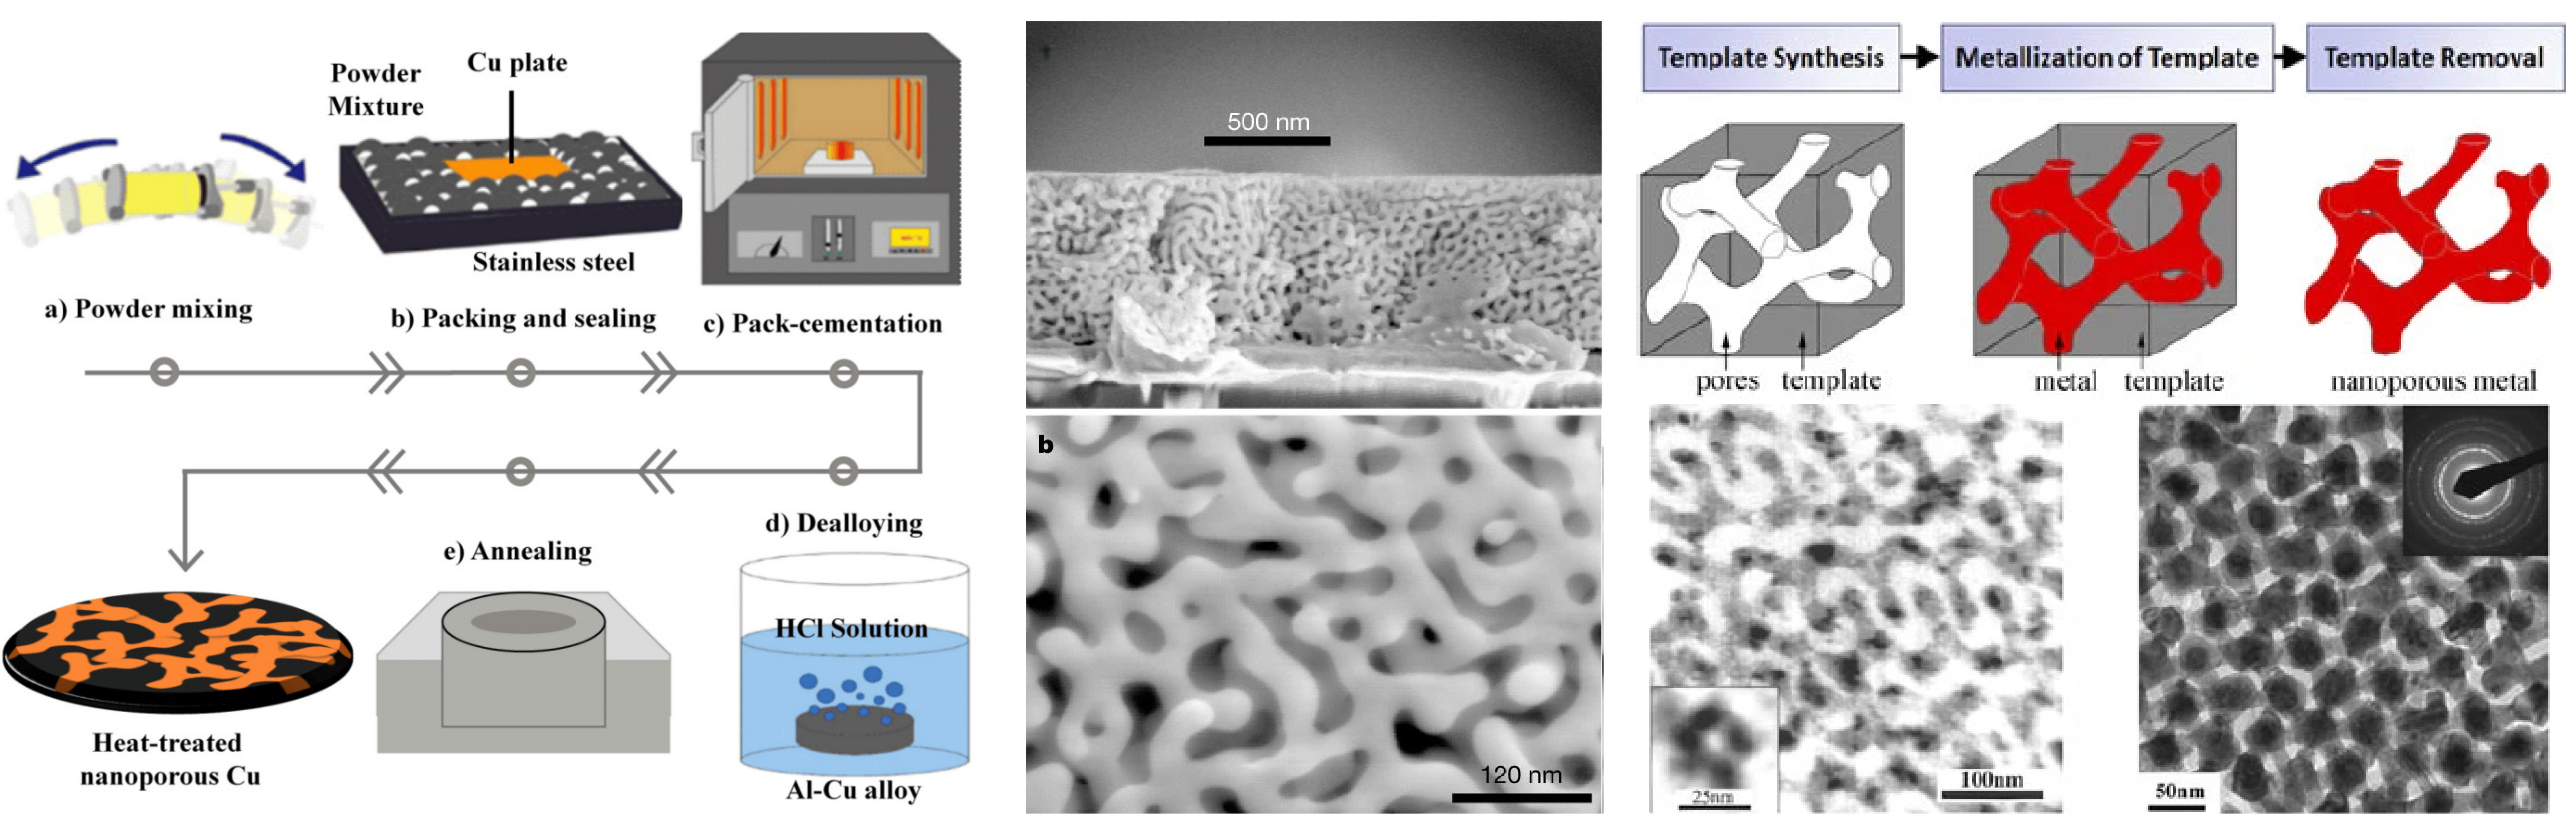
\includegraphics[width=1\linewidth]{photos/how2nanofoam.png}
    \caption{ a) Schematic process of dealloying of an Al-Cu Alloy \cite{Liu2020CuNanofoam}. b) Cross-section of dealloyed Au32$\%$Ag68$\%$ thin film. c) Schematic process and results of template-based fabrication of nanoporous metals \cite{Rebbecchi2018TemplateNanoporousMetals}.}
    \label{fig:how2nanofoam}
\end{figure}
\begin{figure} [H]
    \centering
    \includegraphics[width=0.9\linewidth]{photos/SCBD.png}
    \caption{a) Schematic representation of the two-source SCBD apparatus used in \cite{Profumo2021Neuromorphic}. b) Schematic representation of a nanocomposite Au/ZrOx film-based device.}
    \label{fig:SCBD}
\end{figure}

Metallic nanofoams can be synthesised using various techniques, generally classified into top-down approaches (dealloying \cite{Erlebacher2001Dealloying}, template-assisted methods \cite{Rebbecchi2018TemplateNanoporousMetals, Lee2006Electrodeposition}, some of them shown in Figure \ref{fig:how2nanofoam}) and bottom-up approaches (combustion synthesis \cite{Tappan2005Combustion}, supersonic cluster beam deposition – SCBD \cite{Profumo2021Neuromorphic, Benetti2018Nanometrology}). Dealloying selectively removes components of a binder to achieve controlled porosity; template-assisted methods use a sacrificial skeleton to shape the structure; electrodeposition in porous matrices allows precise control of pores and bonds; SCBD, whose experimental apparatus is shown in Figure \ref{fig:SCBD}, directly assembles metal clusters into three-dimensional nanostructures; combustion synthesis exploits exothermic reactions to generate a porous network. Each technique offers specific advantages in terms of morphological control, scalability and structure quality.






\section{My work}
Modelling thermal transport in metallic systems is a central challenge in modern materials science for a wide range of applications. Local disorder and size effects strongly influence heat transport, making traditional continuum or bulk-based models often insufficient to capture the underlying physics.\bigskip

This thesis studies how the phononic contribution to thermal conductivity varies across a multitude of Au-configurations: from the perfect bulk configuration to highly nanostructured assemblies, including nanopillars and nanofoams. In particular, the presented work explores the impact of porosity-driven defects on the overall thermal conductivity, including randomly distributed vacancies, spherical holes, and central voids, and sees how these initial systems can be used to parametrise assembled nanoparticle structures. 

To quantify the phononic contribution to thermal transport, we employ Equilibrium Molecular Dynamics (EMD) simulations, combining them with the Green–Kubo (GK) method to compute thermal conductivity. The full methodology is detailed in Chapter \ref{chap:md}. GK's method is the one that can also be extended to nanostructured systems, since it does not require a parametrisation of phonons into wave modes, which is not feasible when periodicity is disrupted.\bigskip 

To successfully compute the thermal conductivity, we develop a complete atomistic workflow that includes all stages of the simulation and analysis, extensively described in Chapter \ref{chap:mywork}. This includes the construction and manipulation of atomic configurations using ASE, the execution of EMD simulations in LAMMPS, and the final post-processing analysis. Python was employed for post-processing routines, utilising libraries like NumPy and Pandas to extract heat flux from the simulation output files, compute the autocorrelation functions, and integrate them according to the GK formalism to obtain the thermal conductivity. Additional structural analyses, including coordination numbers and porosity profiles, were also performed to correlate atomic-scale features with thermal transport.\bigskip

Overall, this thesis demonstrates that meaningful estimates of thermal conductivity can be obtained with the GK method even for complex, nanostructured systems that deviate from ideal crystalline assumptions. As summarised in Chapter 4, the results highlight the central role of porosity and local coordination in influencing thermal transport and illustrate how similar atomic fractions arranged in different topologies can lead to different thermal behaviour. 